\documentclass[11pt,a4paper]{article}
\usepackage[margin=2.2cm]{geometry}
\usepackage{graphicx,booktabs,xcolor,array,float}
\usepackage[hidelinks]{hyperref}
\usepackage{fancyhdr}
\pagestyle{fancy}\fancyhf{}
\lhead{34870 Loudspeaker project -- listening test 18 Nov 2026}\rhead{Group 10, System D}\cfoot{\thepage}
\setlength{\parskip}{4pt}\setlength{\parindent}{0pt}
\begin{document}

{\LARGE\bfseries Listening test 18 November: results}\\[2pt]
{\large 34870 Electroacoustics, loudspeaker project, Group 10 (System D), IEC listening room}\\[2pt]
{\small Data: \texttt{listening\_results\_2026-11-18.csv} in this folder (the \texttt{/results.csv} export of the phone
form, blind conditions filled in). Numbers and figures: \texttt{python3 analyze\_listening.py} $\rightarrow$
\texttt{numbers.txt}, \texttt{fig\_*.png}. Test design: \texttt{../ListeningTest\_Operator.pdf} and
\texttt{../ListeningTest\_Questionnaire.pdf}.}

\section*{In one paragraph}
Three listeners rated System D as designed (MiniDSP Out~1 $-5.8$\,dB, tweeter L-pad Rp 8.2\,$\Omega$) at
\textbf{7.75 out of 10} overall. The bass amount was judged \textbf{just right} (0.00 on the $-2\ldots+2$ scale),
and the listeners clearly heard the woofer-level changes in Part~B: the bass-amount ratings rise in step with
the gain. The weak point is the treble. \textbf{Treble smoothness is the lowest-rated attribute} (3.25 of 5,
2.3--2.7 on the two vocal tracks), the treble amount leans towards too much ($+0.33$), and in Part~C the
tweeter 2.9\,dB lower (Rp 3.3\,$\Omega$) was \textbf{preferred by two of three listeners}, with nobody
preferring the design value. Part~C was run with the woofer still at $-3.8$\,dB from Part~B (2\,dB above the
design) for both samples, so it compares the two resistors fairly but not at the design balance. Listening informally after the test, the group itself preferred the woofer much higher, at 0\,dB
(section 7); that is not blind and runs against the listeners' Part~B ratings. With three untrained listeners in one session and one fixed playback order,
these are trends to check against the measurements, not statistically significant results.

\begin{center}\small
\begin{tabular}{@{}>{\raggedright}p{5.6cm}>{\raggedright}p{6.4cm}>{\raggedright\arraybackslash}p{3.6cm}@{}}\toprule
Question & Result & Reading\\\midrule
Overall, as designed (Part A) & 7.75 / 10 (sd 1.6, 12 ratings) & good\\
Bass amount (Part A) & 0.00, just right & keep\\
Treble smoothness (Part A) & 3.25 / 5, lowest attribute; 2.3 and 2.7 on the vocals & weak point\\
Woofer level (Part B) & bass amount $-0.33 / +0.17 / +1.33$ for $-7.8 / -5.8 / -3.8$\,dB & audible, design level fine\\
Tweeter level (Part C, woofer at $-3.8$\,dB) & Rp 3.3\,$\Omega$ preferred 2, no difference 1, Rp 8.2\,$\Omega$ 0 & lower tweeter favoured\\\bottomrule
\end{tabular}
\end{center}

\section*{1\quad The test}
\textbf{Listeners.} Three, all in session 1, one per seat (left, middle, right), submitted 16:17--16:19.
None is a group member, none has listening-test experience, none reported a hearing problem.

\textbf{Parts.} A: the loudspeaker as designed, four tracks (1 Alison Krauss, 2 Stevie Wonder, 3 The Prodigy,
4 Pink Floyd), seven attributes each. B: four samples of tracks 2 and 3 with the woofer channel at
L $-7.8$, D $-5.8$ (design, played twice) and H $-3.8$\,dB; bass amount and overall. C: two samples of tracks 4
and 2 with Rp 8.2\,$\Omega$ (design) and 3.3\,$\Omega$, which on 12 November measured 2.9\,dB lower at
5--15\,kHz; treble amount, smoothness, overall. Part D (vent) was not run.

\textbf{Scales.} Bass and treble amount: $-2$ too little, 0 just right, $+2$ too much. Quality attributes:
1 worst to 5 best. Overall: 0--10. Playback from Spotify through the control panel, Schiit Modi, MiniDSP.

\textbf{Order.} All three listeners sat in session 1, so all heard order row 1: Part B as D, L, D, H and
Part C with Rp 8.2\,$\Omega$ as sample X, i.e. always first.

\textbf{Deviation from the plan.} After Part~B the woofer gain was not set back: it stayed at sample H,
\textbf{Out~1 $-3.8$\,dB}, for both Part~C samples (planned: the design $-5.8$\,dB). Part~C therefore compares
the two resistors at a woofer level 2\,dB above the design.

\section*{2\quad Part A: the loudspeaker as designed}
\begin{figure}[H]\centering
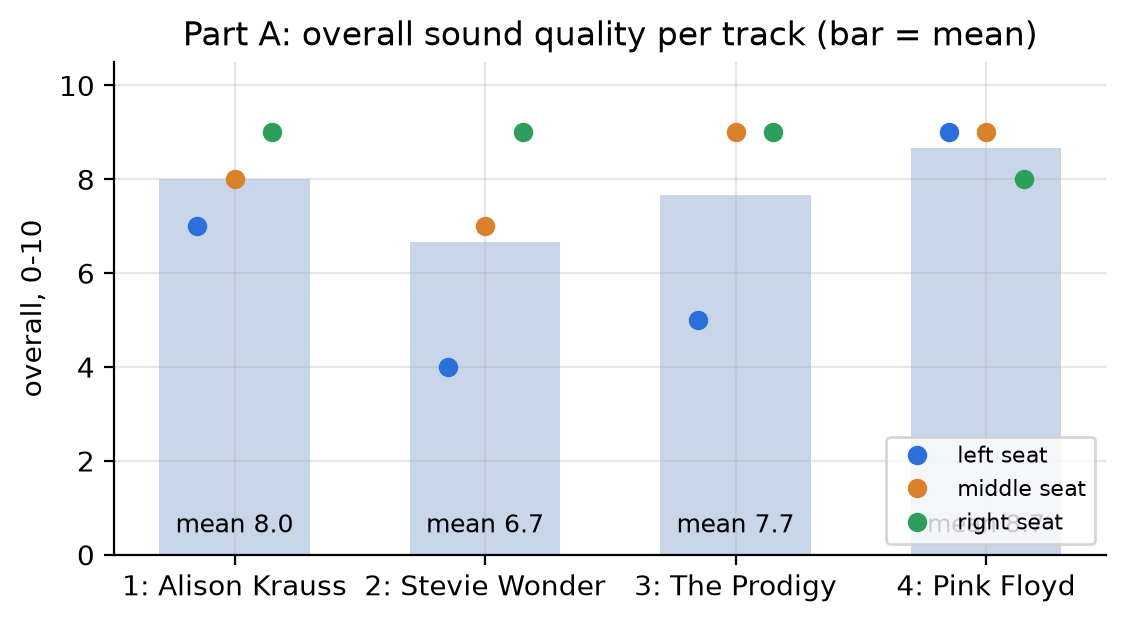
\includegraphics[width=0.78\linewidth]{fig_A_overall.png}\\[2pt]
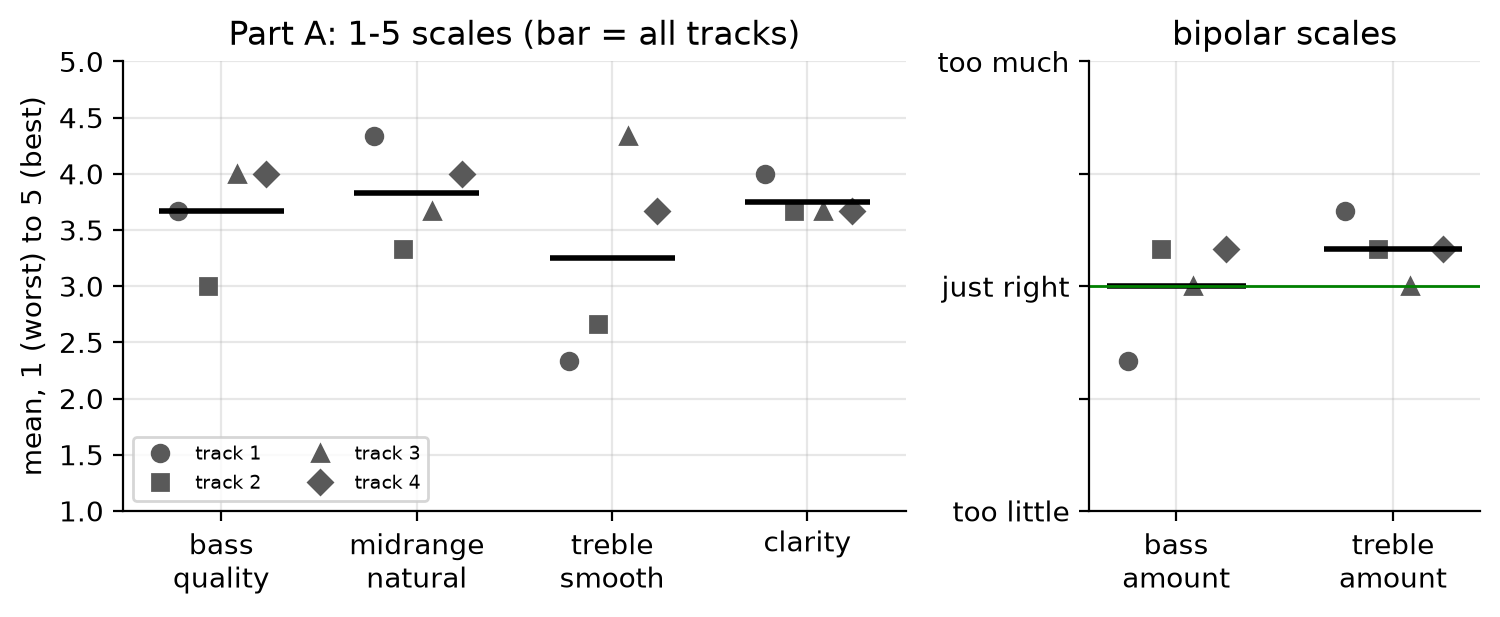
\includegraphics[width=0.95\linewidth]{fig_A_profile.png}
\caption{Top: overall per track, each dot one listener. Bottom: mean per track (markers) and over all tracks
(bars). The green line is ``just right''.}
\end{figure}

\begin{center}\small
\begin{tabular}{@{}lccccc@{}}\toprule
Attribute & Track 1 & Track 2 & Track 3 & Track 4 & All tracks\\\midrule
Bass amount ($-2\ldots+2$) & $-0.67$ & $+0.33$ & $0.00$ & $+0.33$ & $0.00$\\
Bass quality (1--5) & 3.67 & 3.00 & 4.00 & 4.00 & 3.67\\
Midrange natural (1--5) & 4.33 & 3.33 & 3.67 & 4.00 & 3.83\\
Treble amount ($-2\ldots+2$) & $+0.67$ & $+0.33$ & $0.00$ & $+0.33$ & $+0.33$\\
Treble smoothness (1--5) & 2.33 & 2.67 & 4.33 & 3.67 & \textbf{3.25}\\
Clarity (1--5) & 4.00 & 3.67 & 3.67 & 3.67 & 3.75\\
Overall (0--10) & 8.00 & 6.67 & 7.67 & 8.67 & \textbf{7.75}\\\bottomrule
\end{tabular}
\end{center}

The tonal balance is close: bass amount averages exactly ``just right'' and treble amount only $+0.33$.
What stands out is \textbf{treble smoothness on the vocal tracks} (2.33 on track~1, 2.67 on track~2 against
4.33 on the electronic track~3), the pattern of harsh ``s'' sounds, i.e. too much energy in the sibilance
region a few kHz up. Track~2 (Stevie Wonder) is the lowest overall (6.67) and also lowest on midrange
naturalness and bass quality.

\textbf{By seat:} overall left 6.25, middle 8.25, right 8.75; treble amount left $+0.75$, middle $+0.25$,
right $0.00$. The left listener also gave the lowest scores on tracks 2 and 3 (4 and 5, against 8--9 from the
others). With one listener per seat, the seat effect (off-axis treble) cannot be separated from that
listener's taste.

\section*{3\quad Part B: woofer level}
\begin{figure}[H]\centering
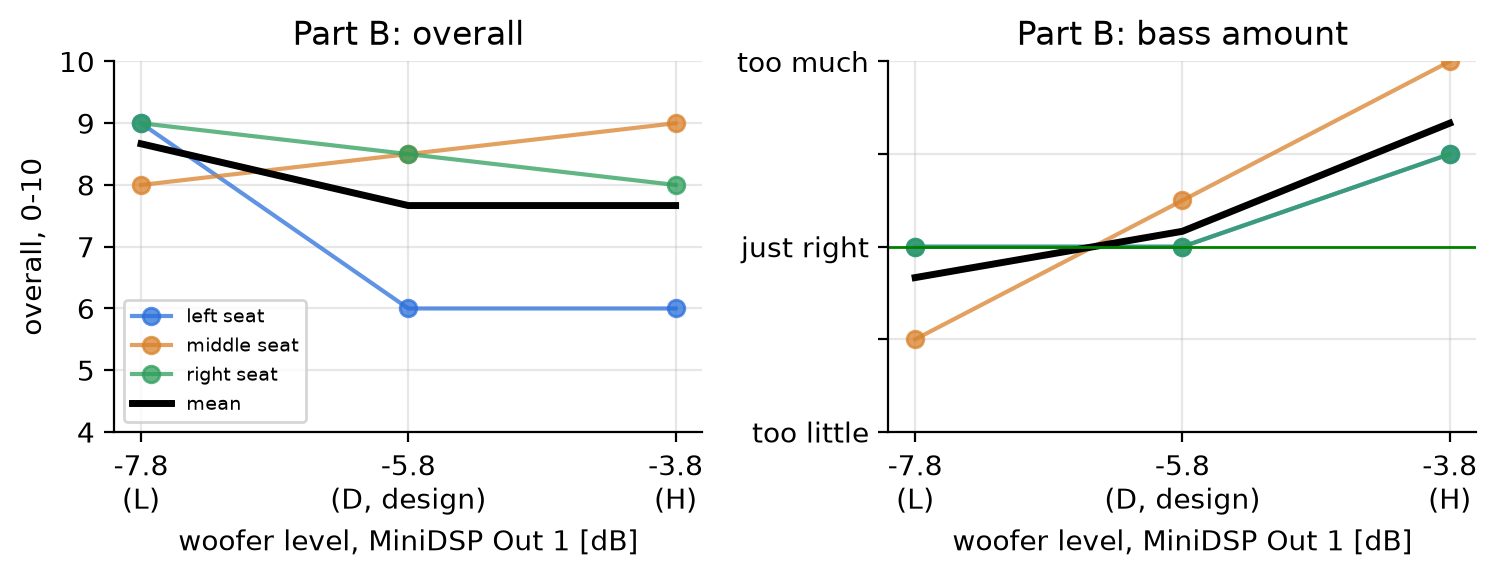
\includegraphics[width=0.95\linewidth]{fig_B_woofer.png}
\caption{Overall and bass amount against the MiniDSP Out~1 gain. Thin lines: listeners (D is the mean of its
two plays); thick line: mean.}
\end{figure}

\begin{center}\small
\begin{tabular}{@{}lcccc@{}}\toprule
Condition & Out 1 gain & Overall (0--10) & Bass amount & Chosen best\\\midrule
L & $-7.8$\,dB & 8.67 (sd 0.58) & $-0.33$ & 1\\
D (design, twice) & $-5.8$\,dB & 7.67 (sd 1.51) & $+0.17$ & 2\\
H & $-3.8$\,dB & 7.67 (sd 1.53) & $+1.33$ & 0\\\bottomrule
\end{tabular}
\end{center}

The listeners heard the changes: \textbf{bass amount rises monotonically} with the woofer gain, from slightly
too little at L to clearly too much at H, and the design level D lands next to ``just right''. Overall does
not separate the conditions: L scores highest on average, but D was picked as best sample twice and L once,
and the two plays of D differed by 1--2 points for the same listener (5/7, 8/9, 8/9), the size of every other
difference in this part. \textbf{Reading:} keep Out~1 at $-5.8$\,dB; up to 2\,dB lower is acceptable,
2\,dB higher is too much bass.

\section*{4\quad Part C: tweeter level}
\begin{figure}[H]\centering
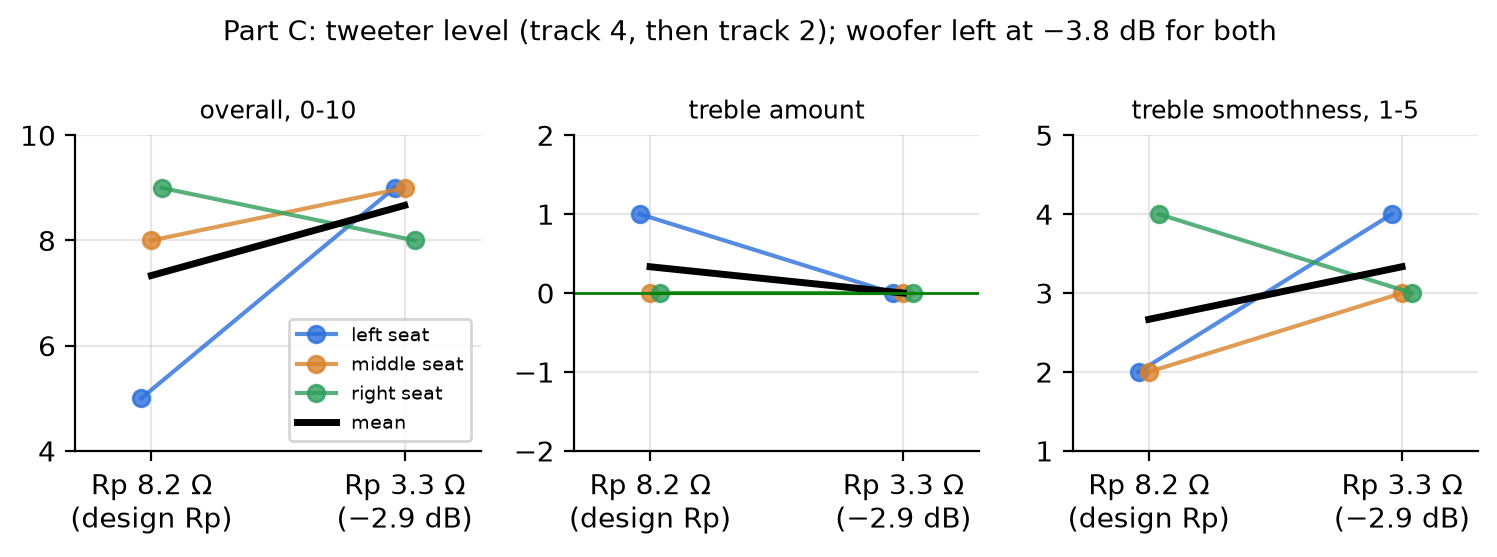
\includegraphics[width=0.95\linewidth]{fig_C_tweeter.png}
\caption{Each listener's two samples joined by a line; thick line: mean. Rp 3.3\,$\Omega$ puts the tweeter
2.9\,dB below the design (measured 12 November). Both samples were played with the woofer at $-3.8$\,dB
(2\,dB above the design), see the note below.}
\end{figure}

\begin{center}\small
\begin{tabular}{@{}lcccc@{}}\toprule
Condition & Overall (0--10) & Treble amount & Treble smoothness (1--5) & Preferred\\\midrule
Rp 8.2\,$\Omega$ (design Rp) & 7.33 (sd 2.08) & $+0.33$ & 2.67 & 0\\
Rp 3.3\,$\Omega$ (tweeter $-2.9$\,dB) & 8.67 (sd 0.58) & $0.00$ & 3.33 & 2\\\bottomrule
\end{tabular}
\end{center}
No difference: 1 (right seat).

Every mean moves the same way as in Part~A: with the tweeter lower, treble amount goes to exactly ``just
right'', smoothness goes up and overall goes up by 1.3 points. Most of the change comes from the left
listener (overall 5 $\rightarrow$ 9, smoothness 2 $\rightarrow$ 4); the middle listener also preferred
Rp 3.3\,$\Omega$ (8 $\rightarrow$ 9), the right listener heard no difference and scored it slightly lower
(9 $\rightarrow$ 8). The design value was played first for everyone, so part of the effect may be order.

\textbf{The woofer was at $-3.8$\,dB in this part.} Both samples had the same woofer level, so the
comparison between the resistors stands. The absolute balance does not: relative to the woofer, the tweeter
was 2\,dB lower than designed with Rp 8.2\,$\Omega$ and 4.9\,dB lower with Rp 3.3\,$\Omega$, while the
tweeter-to-midrange step (2.9\,dB) is unaffected because the midrange is on the other output. That the
listeners still asked for less tweeter, with the bass already 2\,dB up, makes the treble finding stronger,
not weaker. What the woofer change does mean: the ``Rp 8.2\,$\Omega$'' sample is \emph{not} the design sound
(that is Part~A); it is the same setting as sample H in Part~B, which scored 7.67 there against 7.33 here.
A retest at $-5.8$\,dB would settle whether Rp 3.3\,$\Omega$ is still preferred at the design bass level.

\section*{5\quad Estimated responses of the settings that were played}
None of the listening settings was measured with the corrected MiniDSP. The curves below are estimates
from the 12-Nov anechoic runs, built as in \texttt{lab-day/analysis/results\_1112.m}: the woofer channel and
the mid/tweeter channel of one run added with their phases, the doubled Out~2 high-pass divided out, S\_3
for Rp 8.2\,$\Omega$ and S\_4 for Rp 3.3\,$\Omega$ (level-matched on the woofer channel, $+0.01$\,dB). A
different Out~1 gain scales the woofer channel only. Check: the design curve reproduces the 12-Nov figure,
5.5\,dB spread / 1.23\,dB rms from 150\,Hz to 15\,kHz, and Rp 8.2 against 3.3 gives $+2.9$\,dB at
5--15\,kHz. On axis at 2.44\,m in the anechoic chamber, 1/6 octave, 0\,dB = the design's median; the
listening room adds its own bass and reflections, so read the differences between curves, not the
absolute shape. Script: \texttt{estimate\_settings.py}; numbers: \texttt{est\_numbers.txt}.

\begin{figure}[H]\centering
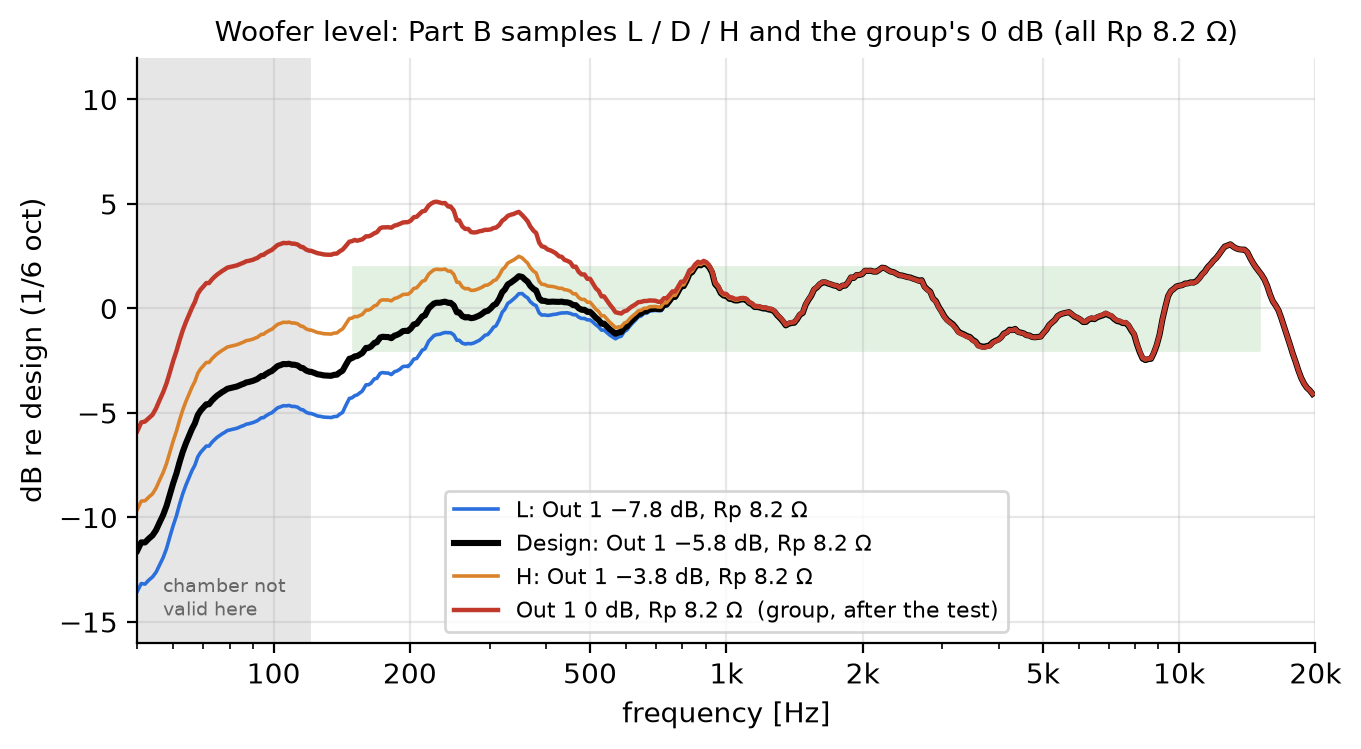
\includegraphics[width=0.92\linewidth]{fig_est_woofer.png}
\caption{Part B samples L, D (design) and H, and the group's 0\,dB from section 7, all with Rp 8.2\,$\Omega$.
The woofer gain moves everything below about 600\,Hz; above 1\,kHz the curves are identical.}
\end{figure}
\begin{figure}[H]\centering
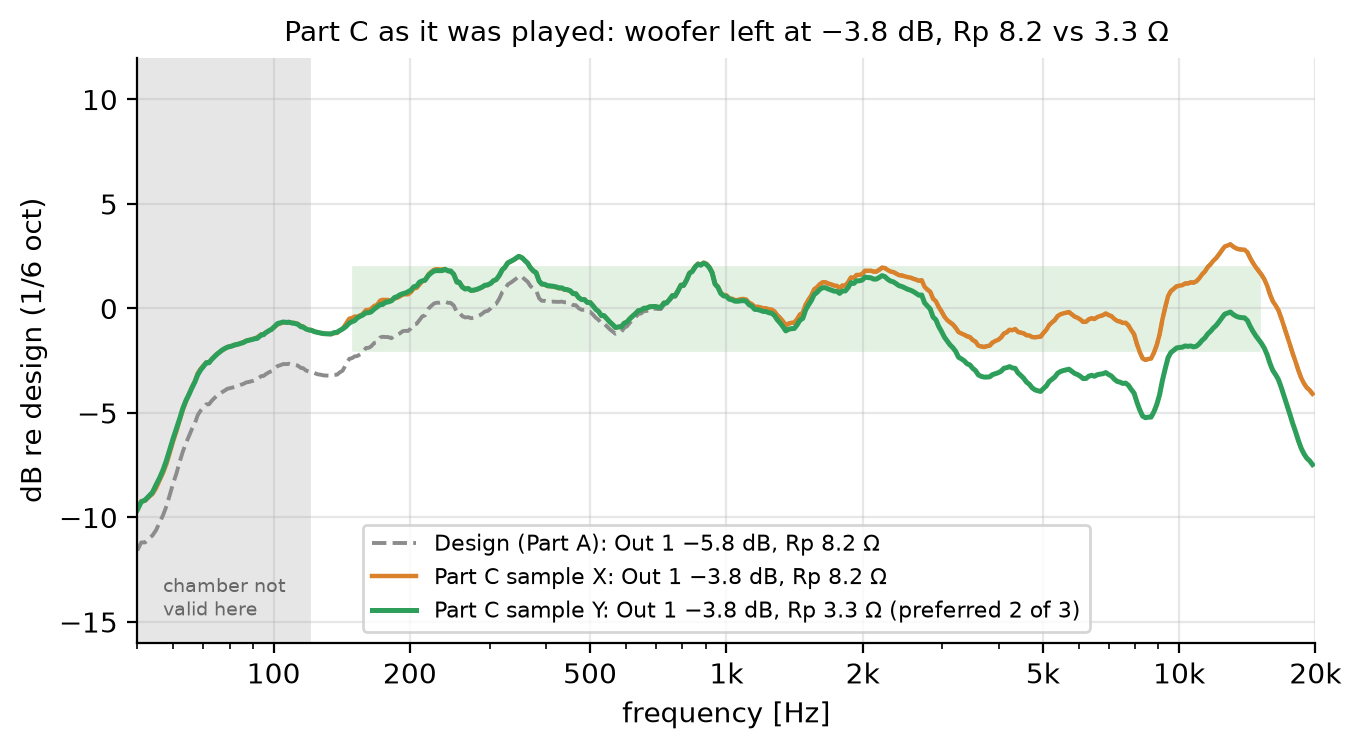
\includegraphics[width=0.92\linewidth]{fig_est_partC.png}
\caption{Part C as it was actually played, with the woofer at $-3.8$\,dB, against the design (dashed).}
\end{figure}

\begin{center}\small
\begin{tabular}{@{}llrrrrrr@{}}\toprule
Setting & Played in & 150--300 & 300--500 & 2--4k & 4--8k & 8--15k & spread\\\midrule
Out 1 $-5.8$, Rp 8.2 (design) & A, B sample D & $-0.8$ & $+0.1$ & $+0.4$ & $-0.9$ & $+1.1$ & 5.5\\
Out 1 $-7.8$, Rp 8.2 & B sample L & $-2.3$ & $-0.5$ & $+0.4$ & $-0.9$ & $+1.1$ & 7.2\\
Out 1 $-3.8$, Rp 8.2 & B sample H, C sample X & $+0.6$ & $+0.9$ & $+0.3$ & $-1.0$ & $+1.1$ & 5.5\\
Out 1 $-3.8$, Rp 3.3 & C sample Y & $+0.7$ & $+0.9$ & $-0.5$ & $-3.5$ & $-2.0$ & 7.7\\
Out 1 0, Rp 8.2 & group, after & $+3.4$ & $+2.6$ & $+0.1$ & $-1.1$ & $+0.9$ & 7.5\\
\bottomrule
\end{tabular}\\[2pt]
{\footnotesize Band medians in dB relative to the same curve's 500\,Hz--2\,kHz median; spread = peak-to-peak
150\,Hz--15\,kHz in dB.}
\end{center}

\textbf{What the curves say.}
\begin{itemize}\setlength{\itemsep}{1pt}
\item \textbf{The treble excess is at the top, not in the classic ``s'' band.} The design's 4--8\,kHz is
slightly low ($-0.9$\,dB); what stands out is a rise to \textbf{+3\,dB around 12--13\,kHz} and a smaller bump
near 2\,kHz (+1.9\,dB). That top-octave peak is the likeliest source of the ``harsh'' and ``annoying treble''
ratings. Rp 3.3\,$\Omega$ removes it (8--15\,kHz $-2.0$\,dB) but also pulls 3--10\,kHz down by about 3\,dB,
so the listeners' preferred sample is not flat either: the spread grows from 5.5 to 7.7\,dB.
\item \textbf{The woofer gain acts on 150--600\,Hz.} The design curve is the flattest there. L leaves a
$-2.3$\,dB shelf at 150--300\,Hz (rated slightly too little bass), H lifts it to $+0.6$ (rated too much).
The listeners' bass ratings follow these few dB closely.
\item \textbf{The group's 0\,dB is a +3 to +5\,dB lower-midrange bulge} (200--400\,Hz) on top of the room's
own bass, with the design tweeter (Rp 8.2\,$\Omega$): the least flat of the woofer settings (7.5\,dB spread
against 5.5 for the design).
\end{itemize}

\section*{6\quad What the listeners wrote}
\begin{itemize}\setlength{\itemsep}{1pt}
\item Left: ``For me the treble is too much, that it can be kind of annoying in track 3'' (Part B, D);
``More smooth'' (B, L); ``Probably it is far too much bass, but I don't find it bad'' (B, H);
``Clarity probably is the weakest point for me. And when treble is high it is so annoying for me'' (last question).
\item Middle: no problem noted in Part A; unsure of their own bass reference (laptop speaker and headphones);
``Louder music can make the sounds more distinct?''
\item Right: ``Some guitar sounds were louder than others''; ``The guitar was slightly louder than the rest'';
D samples ``more balanced''; the intense guitar drew the attention.
\end{itemize}
(Spelling of ``tremble'' corrected to ``treble''; otherwise as written. Full text in \texttt{numbers.txt}.)

\section*{7\quad After the test: the group's own listening}
After the test the group listened to the speaker informally and \textbf{preferred the woofer at Out~1
0\,dB}, i.e. 5.8\,dB above the design and 3.8\,dB above sample H. This is a different kind of evidence from
Parts A--C: not blind, by the people who built the speaker, with the condition known, and without a rating
sheet. The tweeter resistor was the design value, Rp 8.2\,$\Omega$; the tracks played were not recorded.

It also points the other way from the listeners. In Part~B the bass amount rose monotonically with the
woofer gain, and at $-3.8$\,dB it was already rated clearly too much ($+1.33$); nobody heard $-5.8$\,dB as
too little. The two can both be true (different listeners and habits, a different seat or level, music with
less bass than tracks 2 and 3), but this test cannot tell which. If the group wants the woofer higher than
the design, the fair check is a short blind comparison of $-5.8$ against 0\,dB with people outside the group,
on the same tracks, plus an on-axis measurement at 0\,dB to see how far the bass then stands above the
150\,Hz--15\,kHz target.

\section*{8\quad Conclusions for the design}
\begin{enumerate}\setlength{\itemsep}{2pt}
\item \textbf{Bass and woofer level: the test says keep $-5.8$\,dB.} Bass amount is just right as designed,
the listeners track the woofer gain correctly, and $-3.8$\,dB was already too much for them. The group's
informal preference for 0\,dB (section 7) disagrees; settle it blind before changing the design.
\item \textbf{Treble: the one consistent complaint.} Lowest-rated attribute in Part~A, the main topic of the
comments, and the lower tweeter level preferred in Part~C. Worth checking against the 12-Nov on-axis
response. The estimate in section 5 points at the top octave: a +3\,dB rise around 12--13\,kHz and a
small bump near 2\,kHz, while 4--8\,kHz is slightly low. A notch or shelf on the tweeter above about
10\,kHz would remove the peak without the 3\,dB dip that Rp 3.3\,$\Omega$ puts into 3--10\,kHz.
Rp 3.3\,$\Omega$ is the simple fix the listeners favoured; it was
the value before 12 November and measured 2.9\,dB lower. Part~C was heard with the woofer 2\,dB up,
so confirm the choice at the design woofer level before changing it.
\item \textbf{Midrange/guitar:} two comments about the guitar standing out suggest a look at the presence
region (1--4\,kHz) as well.
\end{enumerate}

\section*{9\quad Limits}
Three listeners, one session, all without listening-test experience; one listener per seat, so seat and
listener are confounded; one fixed order for everyone (Part C design value always first); the D repeat shows
a 1--2 point spread within one listener, the same size as most differences here; Part~C was played with the woofer at $-3.8$\,dB instead of
$-5.8$\,dB (left over from Part~B). No test of significance is
meaningful at $n=3$. Part D (vent) was not run. The result is a direction for the design discussion,
supported by the measurements, not a verdict on its own.

\end{document}
